%% Requires compilation with XeLaTeX or LuaLaTeX
\documentclass[10pt,xcolor={table,dvipsnames},t]{beamer}
\usetheme[background=dark]{trigon}
\usepackage{amsmath}
\usepackage{nicefrac}
\usepackage{amssymb}
%\usepackage{enumitem}
\usepackage{braket}
\usepackage{empheq}
\usepackage{color}
\usepackage{keyval}
\usepackage{subcaption}
\usepackage{calrsfs}
\usepackage{hyperref}
\usepackage{eufrak}
\usepackage{transparent}

\captionsetup{font=scriptsize}
\title{Open Quantum System}
\subtitle{
  Lectures: \\ 
  \footnotesize
  \begin{itemize}
      \setlength\itemsep{-0.5em}
    { 
      \transparent{0.4}
    \item[] Last time:
    \item Daniel Manzano, A short introduction to the Lindblad master equation (\textit{all})
    \item Breuer and Petruccione, The Theory of Open Quantum Systems (\textit{ch. 3 - 4.3})
    \item Daniel A. Lidar, Notes on the Theory of Open Quantum Systems (\textit{up to ch. 12})
    }
  \item[] Today:
    \item Breuer and Petruccione, The Theory of Open Quantum Systems (\textit{ch. 3 - 4.3})
    \item Daniel A. Lidar, Notes on the Theory of Open Quantum Systems (\textit{up to ch. 12})
    \item B.Kraus, H.P.Buchler, S. Diehl, A. Kantian, A. Micheli, \& P. Zoller, Preparation of Entangled States by Quantum Markov Processes
    \item Buča, B., Tindall, J. \& Jaksch, D. Non-stationary coherent quantum many-body dynamics through dissipation
    \item Victor V. Albert \& Liang Jiang, Symmetries and conserved quantities in Lindblad master equations
    \item Cameron Booker, Berislav Buča, Dieter Jaksch, Non-stationarity and Dissipative Time Crystals: Spectral Properties and Finite-Size Effects
  \end{itemize}
  \vspace{-1cm}
}
\newcommand{\dt}{\frac{d}{dt}}
\newcommand{\Hint}{H_{\text{int}}}
\newcommand{\outerprod}[2]{\ket{#1}\!\!\bra{#2}}
\newcommand{\tr}[2]{\text{Tr}_{#1}\bigl[#2\bigr]}

\setbeamertemplate{footline}{
  \hbox{%
    \begin{beamercolorbox}[wd=.5\paperwidth,ht=2.5ex,dp=1ex,left]{author in head/foot}%
      %\usebeamerfont{author in head/foot}\insertshortauthor~~(\insertshortinstitute)
    \end{beamercolorbox}%
    \begin{beamercolorbox}[wd=.5\paperwidth,ht=2.5ex,dp=1ex,right]{title in head/foot}%
    \end{beamercolorbox}}%
  \vskip0pt%
}

\newlength\mytemplen
\newsavebox\mytempbox

\newcommand\mybluebox{%
    \@ifnextchar[%]
       {\@mybluebox}%
       {\@mybluebox[0pt]}}

\definecolor{myblue}{rgb}{.8, .8, 1}

\def\@mybluebox[#1]{%
    \@ifnextchar[%]
       {\@@mybluebox[#1]}%
       {\@@mybluebox[#1][0pt]}}

\def\@@mybluebox[#1][#2]#3{
    \sbox\mytempbox{#3}%
    \mytemplen\ht\mytempbox
    \advance\mytemplen #1\relax
    \ht\mytempbox\mytemplen
    \mytemplen\dp\mytempbox
    \advance\mytemplen #2\relax
    \dp\mytempbox\mytemplen
    \colorbox{myblue}{\hspace{1em}\usebox{\mytempbox}\hspace{1em}}}

\begin{document}

\begin{frame}
  \titlepage
\end{frame}


\begin{frame}{Last time}
\begin{itemize}
    \item<1-> Derivation of the Lindblad equation via different approximations:
      \begin{itemize}
        \item<2-> Von Neumann evolution equation, $\Hint=\sum_k S_k \otimes B_k$ $\rightarrow$ Weak coupling, Born, Markov \& Rotating wave $\rightarrow$ Redfield equation\\
          \textit{Note: no stationarity of the system was assumed!}
        \item<3-> Yielding (Schrodinger pic.): 
        \begin{equation}
          \begin{split}
            \dt \rho(t) &= [H+H_\text{LS}, \rho(t)] + \\
                        +&\sum_{k,l, \omega} \gamma_{k,l}(\omega) \Bigl[S_l(\omega)\rho(t)S_k^\dag(\omega) - \frac{1}{2}\bigl\{ S_k^\dag(\omega) S_l(\omega), \rho(t) \bigr\}\Bigr]
          \end{split}
        \end{equation}
      \item<4-> With $\gamma_{k,l}$, $\pi_{k,l}$ - defined via $\Gamma_{k,l}(\omega)$'s real and imaginary parts.
          \begin{equation}
            \begin{split}
              H_\text{LS} &= \sum_{\omega, k,l}\pi_{k,l}(\omega)S_k^\dag (\omega) S_l(\omega)\\
              \Gamma_{k,l}(\omega) &= \int_0^\infty e^{i\omega s} \tr{B}{B_k^\dag(t) B_l(t-s) \rho_B(0)}
            \end{split}
          \end{equation}
      \end{itemize}
\end{itemize}
\end{frame}

\begin{frame}{}
\begin{itemize}
  \item<1-> With the operators $S_k(\omega)$ defined via 
    \begin{equation}
      S_k(\omega) = \sum_{\epsilon' - \epsilon = \omega} \Pi_\epsilon S_k \Pi_{\epsilon'} \equiv \sum_{\epsilon' - \epsilon = \omega}\outerprod{\epsilon}{\epsilon} S_k \outerprod{\epsilon'}{\epsilon'}
    \end{equation}
  \item<2-> Yielding a time evolution (Dirac's pic) in the form 
    \begin{equation}
      \Hint(t) = \sum_{\alpha, \omega} e^{-i\omega t} S_\alpha (\omega) \otimes B_\alpha (t)\;, \quad B_\alpha(t) = e^{iH_B t}B_\alpha e^{-iH_B t}
    \end{equation}
  \item<3-> $$\dt \rho(t) = [H+H_\text{LS}, \rho(t)] + \sum_{k,l, \omega} \gamma_{k,l}(\omega) \Bigl[S_l(\omega)\rho(t)S_k^\dag(\omega) - \frac{1}{2}\bigl\{ S_k^\dag(\omega) S_l(\omega), \rho(t) \bigr\}\Bigr]$$
            which we can diagonalize over $(k,l)$, by defining $\gamma(\omega) = U \varSigma(\omega) U^\dag$, with $\varSigma(\omega) = \text{Diag}(\varsigma_k(\omega))$ and the transformation of 
            the jump operators - $L_k(\omega) = \sum_l U_{lk}S_l(\omega)$. Yielding
\end{itemize}
\begin{block}{Lindblad}<4->
              $\dt \rho(t) = [H+H_\text{LS}, \rho(t)] + \sum_{\omega} \sum_k \varsigma_k(\omega)\Bigl[L_k(\omega)\rho(t)L_k^\dag(\omega) - \frac{1}{2}\bigl\{ L_k^\dag(\omega)L_k(\omega), \rho(t) \bigr\}\Bigr]$
          \end{block}
\end{frame}

\begin{frame}{Dissipation \& Decoherence}
  \begin{block}{\textit{Decoherence \& Dissipation}}
     Processes, through which a quantum system will loose its quantum properties over time, via a coupling to the environment.
  \end{block}
\begin{itemize}
    \begin{itemize}
      \item<2-> Loss of energy - \textbf{dissipation}
      \item<3-> Loss of coherence - \textbf{decoherence}
        \begin{itemize}
          \item<3-> Loss of information 
          \item<3-> Loss of entanglement
          \item<3-> Loss of correlations, superpositions
        \end{itemize}
      \item<4-> Examples of such phenomena
        \begin{itemize}
          \item<4-> Energy shift and relaxation to the ground state of the system.
          \item<5-> Decay of the off-diagonal terms of the density operator, leading to loss of superpositions.
            In the spin-boson model, a possible solution for $\rho(t)$
            $$\rho_{01}(t)\propto \exp\biggl( -Ct\tau \int_0^{\omega_c} d\omega \text{ sinc}^2(\nicefrac{\omega \tau}{2}) \biggr)$$
          \item<5-> Or, in contrary, pure states can loose their purity due to the effect of decoherence.
        \end{itemize}
        \item<6-> Note: relaxation mechanisms are always present in practice.
    \end{itemize}
\end{itemize}
\end{frame}

\begin{frame}{Steady state and stationarity}
  \begin{block}{Why steady state?}
    \centering
    \;\underline{Eigenstate thermalization hypothesis} + \underline{ergodicity} \hfill $\rightarrow$ \hfill \underline{Steady state system}\;
  \end{block}
  \begin{columns}
    \begin{column}{0.8\textwidth}
      \begin{itemize}
        \item<2-> \textsl{\underline{Question: } are there some systems so that this steady state is not achieved? If yes, 
          what are those states and conditions? Do they belong to some isolated subspace of the Hilbert space $\tilde{\mathcal{H}} \in \mathcal{H}$}\;? 
        \item<3-> For the most widely used cases, one supposes \textbf{ergodicity}, meaning the state explores the accessible state space, 
          as illustrated in \textit{figure (a)}, before reaching the supposed stationarity. 
      \end{itemize}
    \end{column}
    \begin{column}{0.2\textwidth}
      \only<3->{
  \begin{figure}
    \centering
      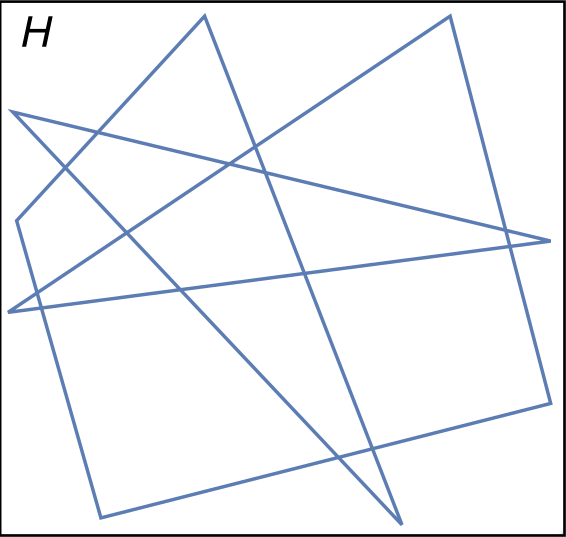
\includegraphics[width=\textwidth]{./ergodic.png}
      \caption{Illustration of ergodicity. \footnote[frame]{Buča, B., Tindall, J. \& Jaksch, D. Non-stationary coherent quantum many-body dynamics through dissipation}}
      \label{fig:entire_phase_space}
  \end{figure}
}

  \end{column}
\end{columns}
\end{frame}

\begin{frame}{Steady state and stationarity}
      \begin{itemize}
        \item<1-> In fact, it \textbf{is possible} to consider the microscopic properties $\mathcal{L}$, such that
          $$\exists \quad \Bigl\{ \{\varphi_m, \ket{\varphi_m}\} \; \vert \; \mathcal{L}\ket{\varphi_m}=\varphi_m \ket{\varphi_m} \text{ and } \{\varphi_m\}\in \sigma(\mathcal{L})  \Bigr\} $$
          meaning, that there can exist a decoherence-free subspace.
      \end{itemize}
            \only<2->{
            \begin{beamercolorbox}[wd=\textwidth, rounded=false, shadow=false, sep=0.05cm]{block body}
              \centering
              Thus, in some cases, even when coupled to the environment, 
              the system can undergo non-stationarity, which will not be the case using 
              the \textit{classical} ETH or ergodic assumptions.
            \end{beamercolorbox}
          }
          \begin{columns}
            \begin{column}{0.75\textwidth}
              \begin{itemize}
                \item<3-> Symmetry-preserving dissipation eliminates \textit{non-coherent}
                  eigenkets.
                \item<3-> Dark Hamiltonian $\mathfrak{H}$ - driver of the \textit{non-decaying}
                  subspaces. 
              \end{itemize}
            \end{column}
            \begin{column}{0.25\textwidth}
              \only<4->{
              \begin{figure}
                \begin{center}
                  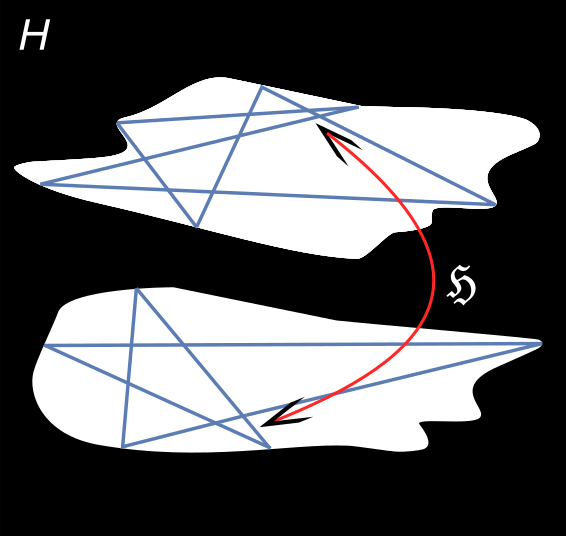
\includegraphics[width=0.7\textwidth]{./non_ergodic.png}
                  \caption{Decoherence-free subspaces, driven by $\mathfrak{H}$.\footnote[frame]{\tiny Buča, B., Tindall, J. \& Jaksch, D. Non-stationary coherent quantum many-body dynamics through dissipation}}
                \end{center}
              \end{figure}
            }
            \end{column}
          \end{columns}
\end{frame}

\begin{frame}{Steady state and stationarity}
  \only<1-2>{
            \begin{beamercolorbox}[wd=\textwidth, rounded=false, shadow=false, sep=0.05cm]{block body}
              \centering
              How to identify those DF - \textbf{decoherence-free subspaces}?
            \end{beamercolorbox}
          }
          \only<2->{
            \begin{beamercolorbox}[wd=\textwidth, rounded=false, shadow=false, sep=0.05cm]{block body}
              \centering
              $\dt \rho(t) = \mathcal{L}\rho(t) = -[H,\rho(t)] + \sum_{\mu}(2c_\mu \rho c_{\mu}^\dag - \{c_\mu c_\mu^\dag,\rho\})$\\
              $\dot{\rho}=\mathcal{L}\rho = \mathcal{E}(\rho)-Q\rho - \rho Q  ,\quad \mathcal{E}\equiv 2\sum_lg_lc_l\rho c_l^\dag, \quad Q\equiv P-iH, \quad P\equiv \sum_l g_l c_l^\dag c_l$
            \end{beamercolorbox}
          }
          \begin{columns}
            \begin{column}{0.75\textwidth}
      \begin{itemize}
        \item<3-> For a steady-state $\rho_\infty$, one clearly has $\mathcal{L}\rho_\infty = 0$
        \item<4-> Density $\rho_n$ non stationary, if the corresponding eigenvalues $\varrho_n$ are purely imaginary.
          \begin{equation}
            \begin{split}
              \mathcal{L}\rho_n &= \varrho_n \rho_n \\
                                &= -i \mathfrak{H}\rho_n = -i\lambda_n \rho_n\;, \quad \lambda\in \mathbb{R}
          \end{split}
          \end{equation}
      \end{itemize}
    \end{column}
    \begin{column}{0.25\textwidth}
      \only<4->{
      \begin{figure}
        \centering
        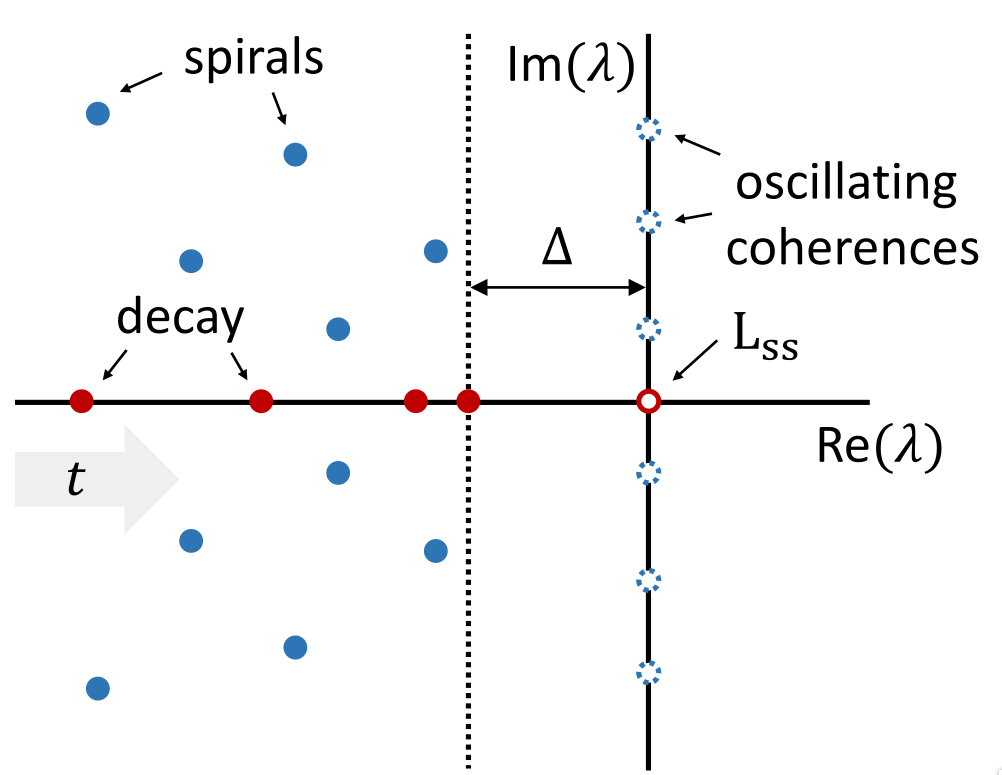
\includegraphics[width=0.7\textwidth]{./eigenvalues_lind.png}
        \caption{Meaning of eigenvalues of $\mathcal{L}$.}
      \end{figure}
    }
  \end{column}
  \end{columns}
\end{frame}

\begin{frame}{Non-dissipative subspaces}
    Let $\ket{\Psi}$ - a pure state, that is \textbf{not} affected by dissipation. Then, 
  \begin{itemize}
    \item<1-> $\ket{\Psi} \in \text{Ker}(P) \equiv \bigl\{ \ket{\Psi} \;\; \vert\;\;\; \hat{c}_l \ket{\Psi}=0 \bigr\} = \text{Ker}(P)\bigcap \text{EigSp}(H) \equiv \mathcal{H}_{ND} $
    \item<2-> Meaning that if for a density operator $\rho$, such that  
      \begin{equation}
        \text{Range}(\rho) = \text{span}(\{\ket{\varphi_i}\}) \;\text{ ,with } \{\varphi_i\} \in \mathcal{H}_{ND}
    \end{equation}
    will represent a stationary state. We call $\{\varphi_i\}$ - dark states.
  \item<3-> We want to define the dark Hamiltonian $\mathfrak{H}$, that
    \begin{itemize}
      \item<4-> $\text{EigSp}(\mathfrak{H})=\{\ket{\varphi_i}\}$ such that $\ket{\varphi_m}\perp \ket{\varphi_n}$ 
      \item<4-> $\mathfrak{H}\outerprod{\varphi_m}{\varphi_n}=(\omega_m-\omega_n) \outerprod{\varphi_m}{\varphi_n}$
      \item<4-> For $\rho_{nm} = \outerprod{\varphi_m}{\varphi_n}$, \; $\Tr{}{\rho_{nm}^\dag \rho_{n'm'}}=\delta_{nm}\delta_{n'm'}$
      \item<4-> Hermicity - $\mathfrak{H}=\mathfrak{H}^\dag$
    \end{itemize}
  \end{itemize}
\end{frame}

\begin{frame}{Non-dissipative subspaces}
  \only<1->{
  There are multiple theorems giving precisions on the \textit{Dark states}. 
}
\only<2-3>{
  \begin{block}{Theorem: conditions stationarity}
    The set $\{\varphi_m\} \in \text{EigSp}(\mathfrak{H})$ with $\ket{\varphi_m} \perp \ket{\varphi_n}$ IFF
    \begin{itemize}
      \item $Q^\dag \ket{\varphi_n}=\lambda \ket{\varphi_n}\;,\quad \forall n$
      \item $c_k\ket{\varphi_n} = \lambda_{kn} \ket{\varphi_n} \quad$, with $\sum_l \gamma_l\vert \lambda_{ln}\vert^2 = \text{Re}(\lambda_n)$
      \item Relations between $\lambda_{kn}$ and $\gamma_k$:
        $$
        \text{Re}\biggl[ \sum_k \gamma_k\Bigl( 2\lambda_{kn}\lambda_{km}^* - 
        |\lambda_{kn}|^2 - |\lambda_{km}|^2 \Bigr) \biggr] = 0 \qquad \forall n,m
        $$
      \item<3-> Corollary for eigenvalues $\omega_{i}$ for the dark Hamiltonian $\mathfrak{H}$:
        \begin{equation}
          \omega_n - \omega_m = \text{Im}\biggl[ \sum_k 2\gamma_k \lambda_{kn}\lambda_{km}^*
            - \bra{\varphi_m}H\ket{\varphi_n}
          \biggr]
        \end{equation}
    \end{itemize}
  \end{block}
}
\only<4->{
  \begin{block}{Theorem: conditions stationarity}
    If there exists no subspace $\mathcal{S}\subseteq \mathcal{H}$ with
    $\mathcal{S} \perp \mathcal{H}_{ND}$ such that 
    $\hat{c}_l(\mathcal{S}) \subseteq \mathcal{S}, \;\; \forall \hat{c}_l$ 
    , then the only oscillating coherences are the dark states, 
    in the form $\outerprod{\varphi_n}{\varphi_m}$, such that $\{\ket{\varphi_n}\} \in \mathcal{H}_{DS}$ 
    defined above.
  \end{block}
}
\only<5->{
  \begin{itemize}
    \item The notations used up to now do \textbf{not} correspond to the one used previously, when 
      defining the $\mathcal{L}$ equation via the spectrum $\omega \in \sigma(H_S)$
  \end{itemize}
}

\only<6->{
  \begin{itemize}
    \item Example of change of notation: $\sum_\mu \mapsto \sum_k\sum_\omega$. 
  \end{itemize}
}
\end{frame}

\begin{frame}{A more general case - non-stationarity}
  \begin{itemize}
    \item<1-> The dark Hamiltonian $\mathfrak{H}$ does not need to be Hermitian in general
    \item<2-> How to find $\rho$, such that, $\mathcal{L} \rho \neq 0$?
  \end{itemize}
  \only<3->{
  \begin{block}{Condition:}
    This is realized, if 
    $\exists A \; : \; [H, A]=-\lambda A \;\; \text{and}\;\; [c_\mu, A]=[c_\mu^\dag, A]=0 \;\;\; \text{with}\;\; \lambda \in \mathbb{R}$
  \end{block}
}
  \only<4->{
  \begin{block}{Corollary:}
    As a consequence, $\exists \rho_{mn} \equiv A^n \rho_{\infty} (A^m)^\dag \;\; m,n\in \mathbb{Z}$ and $\mathcal{L}\rho_{mn}=i(m-n)\lambda \rho_{mn}$
  \end{block}
}
\only<4->{
  \begin{figure}
    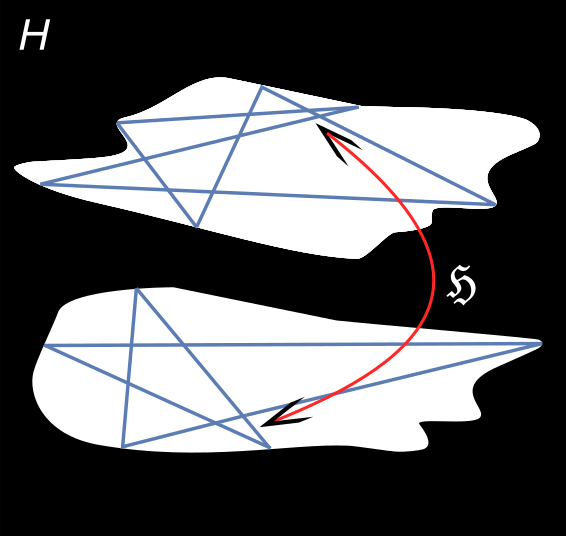
\includegraphics[width=0.25\textwidth]{./non_ergodic.png}
  \end{figure}    
}
\end{frame}

\begin{frame}{Recap \& terminology}
  \begin{itemize}
    \item<1-> Decoherence, dissipation - loss of quantum properties 
    \item<2-> Steady-state \;$\rightleftarrows$\; ergodicity \& ETH
    \item<3-> \textbf{Dark states} $c_k\ket{\varphi_n}=0 \;\forall n$ - invisible for decoherence. 
    \item<4-> $\rho_{mn} = \outerprod{\varphi_m}{\varphi_n} \in \text{EigSp}(\mathcal{L})$ \;\; with eigenval. \;$\lambda_{mn} = -i(E_n - E_m)$
    \item<5-> Mixed coherences $\rho_{nm}= (A^\dag)^n \rho_\infty A^m$ also in $\text{EigSp}(\mathcal{L})$ with 
      eigenvalues $\lambda_{nm}^j=i(n-m)\omega_j$, with $\omega_jA_j = [H,A_j]$
  \end{itemize}
\only<6->{
  \begin{block}{Remark}
    \centering
    It is important to distinguish the \textbf{\underline{mixed coherences}} and \textbf{\underline{decoherence free subspace of dark space}}. 
    \\Namely, 
    $\hat{c}_l\ket{\varphi_n}=0$ for dark states and $\hat{c}_l \rho_{nm} \hat{c}_l^\dag \neq 0$
  \end{block}
}
\only<7->{
  \begin{block}{Corollary}
    The mixed coherence states' evolution depends on dissipative processes.
  \end{block}
}
\end{frame}
\end{document}






